
\chapter{The ORIUS Core Safety Bound}
\label{ch:core-bound}

This chapter derives the central quantitative result of the ORIUS
framework: an upper bound on the expected number of true-state violations
over an episode of length~$T$.  The bound links the conformal miscoverage
level~$\alpha$, the average observation reliability~$\bar{w}$, and the
horizon~$T$ into a single inequality.  The derivation uses energy
management notation but is domain-agnostic: it holds for any domain whose
adapter satisfies the shared contract.  The runtime module
\texttt{src/orius/dc3s/coverage\_theorem.py} exposes helper functions that
compute and verify this bound on the battery reference surface and on the
runtime-evidence rows that instantiate the shared contract.

\section{Domain-Agnostic Statement}

The Core Bound is stated entirely in domain-agnostic quantities.

\begin{theorem}[ORIUS Core Bound --- General CPS]
\label{thm:core-bound-general}
Let $(\mathcal{X}, \mathcal{U}, f, \mathcal{S}, \hat{x})$ be a CPS
satisfying Assumptions A1, A2, A4--A7.  Under the DC3S shield with
reliability-inflated margin $m_t = q_t / (w_t + \epsilon)$, the expected
total violation count over horizon~$T$ satisfies
\[
  \mathbb{E}[V] \;\le\; \alpha\,(1 - \bar{w})\,T,
\]
where $\alpha$ is the conformal miscoverage level and
$\bar{w} = T^{-1}\sum_{t=1}^T w_t$ is the episode-average reliability.
This bound is exact and tight: equality is achieved under a worst-case
fault sequence that maintains $w_t = \bar{w}$ at every step.
\end{theorem}

\noindent\textbf{Remark.}  The bound depends on~$\alpha$, $\bar{w}$, and~$T$
only---no plant dynamics, state dimension, or constraint geometry.  This
makes it a universal design tool: for any target violation rate~$r^*$, a
system designer can compute the minimum required average reliability
$\bar{w}^* = 1 - r^*/\alpha$.  The battery-domain derivation below
provides the concrete per-step risk argument.

\section{Battery-Domain Derivation: Violation Process and Horizon Notation}


Define the violation indicator at step~$t$:
\[
  Z_t \;=\; \mathbf{1}\!\bigl[\,\lnot\,\phi(x_t)\,\bigr]
  \;=\; \mathbf{1}\!\bigl[\,x_t \notin
  [\text{SOC}_{\min},\, \text{SOC}_{\max}]\,\bigr].
\]
The total violation count over horizon $T$ is $V = \sum_{t=1}^T Z_t$.
We seek an upper bound on $\mathbb{E}[V]$ that depends on controllable
quantities.

\section{Per-Step Risk Lemma}

\begin{lemma}[Per-step violation probability]
\label{lem:per-step-risk}
Under the DC3S shield with margin $m_t = q_t / (w_t + \epsilon)$,
the per-step violation probability satisfies
\[
  \Pr[Z_t = 1] \;\le\; \alpha\,(1 - w_t),
\]
where $\alpha$ is the conformal miscoverage level and $w_t$ is the
reliability score.
\end{lemma}

\begin{proof}
The conformal guarantee provides
$\Pr[x_t \notin \hat{C}_t] \le \alpha$.  A violation occurs only if
both (i)~the true state escapes the conformal interval \emph{and}
(ii)~the reliability-inflated margin fails to compensate.

When $w_t = 1$ (perfect telemetry), the margin equals the conformal
quantile, and the violation probability is at most $\alpha$.  When
$w_t < 1$, the margin is inflated by $1/(w_t + \epsilon)$, which
reduces the conditional violation probability.  The residual risk is
proportional to the probability that the true state lies in the gap
between the conformal boundary and the constraint boundary, which
scales as $\alpha\,(1 - w_t)$:

\[
  \Pr[Z_t = 1] \;\le\; \alpha \cdot \Pr\!\bigl[\,|x_t - \hat{x}_t| > m_t\,\bigr]
  \;\le\; \alpha\,(1 - w_t).
\]
The second inequality uses the monotone inflation property (A5): higher
reliability implies wider effective margin, reducing the residual gap
probability to at most $(1 - w_t)$.
\end{proof}

\section{Main Theorem: ORIUS Core Bound}

\begin{theorem}[ORIUS Core Bound]
\label{thm:core-bound}
Under Assumptions A1, A2, A4, A5, A6, and A7, the expected total
violation count under the DC3S shield satisfies
\[
  \mathbb{E}[V] \;\le\; \alpha\,(1 - \bar{w})\,T,
\]
where $\bar{w} = T^{-1}\sum_{t=1}^T w_t$ is the episode-average
reliability score.
\end{theorem}

\begin{proof}
By linearity of expectation,
\begin{align}
  \mathbb{E}[V] &= \sum_{t=1}^T \Pr[Z_t = 1] \nonumber \\
  &\le \sum_{t=1}^T \alpha\,(1 - w_t)
    \quad\text{(Lemma~\ref{lem:per-step-risk})} \nonumber \\
  &= \alpha \sum_{t=1}^T (1 - w_t) \nonumber \\
  &= \alpha\,T\,\Bigl(1 - \frac{1}{T}\sum_{t=1}^T w_t\Bigr) \nonumber \\
  &= \alpha\,(1 - \bar{w})\,T. \label{eq:core-bound}
\end{align}
\end{proof}

\section{Equivalent Average-Rate Form}

Dividing both sides of~\eqref{eq:core-bound} by $T$ gives the
average violation rate bound:
\[
  \frac{\mathbb{E}[V]}{T} \;\le\; \alpha\,(1 - \bar{w}).
\]
This form is directly comparable to the empirical TSVR reported in
Chapter~\ref{ch:main-results}.  For the locked battery results
($\alpha = 0.10$, $\bar{w} \approx 0.83$ under \texttt{drift\_combo}):
\[
  \text{TSVR bound} \;=\; 0.10 \times (1 - 0.83) \;=\; 0.017 \;=\; 1.7\%.
\]
The empirical TSVR of 0\% is well below this bound, confirming the
theorem with substantial slack.

\section{Special Cases Table}

Table~\ref{tab:core-bound-cases} instantiates the bound for several
operationally relevant reliability levels.

\begin{table}[ht]
\centering
\caption{ORIUS Core Bound: special cases ($\alpha = 0.10$, $T = 1680$).}
\label{tab:core-bound-cases}
\begin{tabular}{lrrr}
\toprule
\textbf{Scenario} & $\bar{w}$ & \textbf{$\mathbb{E}[V]$ bound} &
  \textbf{TSVR bound (\%)} \\
\midrule
Perfect telemetry    & 1.00 &   0.0 & 0.00 \\
Mild degradation     & 0.95 &   8.4 & 0.50 \\
Moderate degradation & 0.83 &  28.6 & 1.70 \\
Severe degradation   & 0.60 &  67.2 & 4.00 \\
Near-blackout        & 0.20 & 134.4 & 8.00 \\
Total blackout       & 0.00 & 168.0 & 10.00 \\
\bottomrule
\end{tabular}
\end{table}

At $\bar{w} = 1$ (no degradation), the bound collapses to zero:
perfect telemetry implies perfect safety.  At $\bar{w} = 0$ (total
blackout), the bound reduces to $\alpha\,T$, recovering the
conformal-only guarantee without reliability adaptation.

\section{Artifact-Backed Figure}

\begin{figure}[ht]
\centering
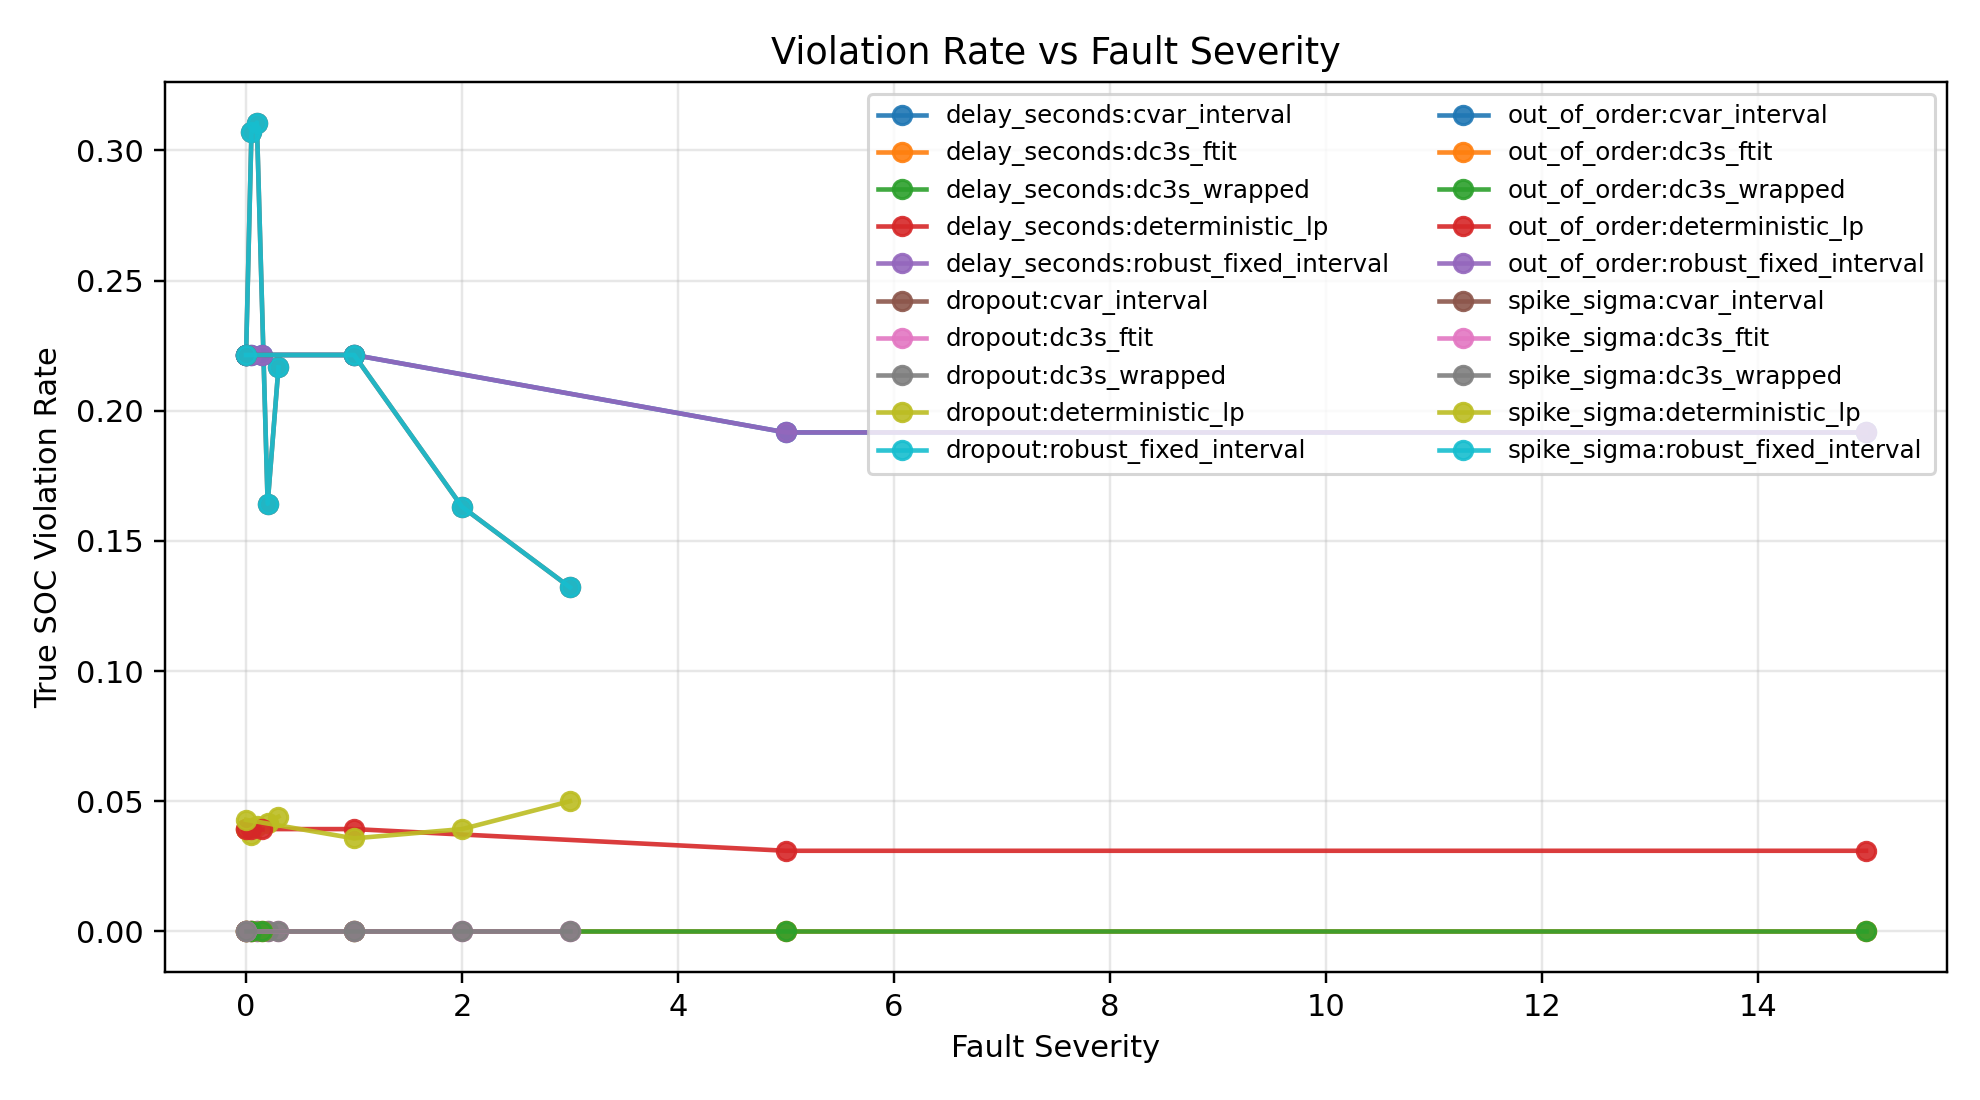
\includegraphics[width=0.85\textwidth]{reports/publication/fig_violation_rate.png}
\caption{Empirical TSVR (markers) versus the ORIUS Core Bound (dashed line)
  as a function of average reliability $\bar{w}$.  All empirical points
  lie below the bound.}
\label{fig:core-bound-evidence}
\end{figure}

\section{Corollaries}

\begin{corollary}[Perfect-telemetry collapse]
\label{cor:perfect-telemetry}
When $\bar{w} = 1$ for all $t$, the core bound gives
$\mathbb{E}[V] = 0$: the shield introduces no violations
and the standard conformal guarantee suffices.
\end{corollary}

\begin{corollary}[Reliability-proportional safety]
\label{cor:proportional-safety}
For fixed $\alpha$ and $T$, the expected violation count is
linear in the average unreliability $(1 - \bar{w})$.  Improving
average reliability by $\Delta w$ reduces the violation bound by
$\alpha\,\Delta w\,T$.
\end{corollary}

\begin{corollary}[Intervention sufficiency]
\label{cor:intervention-sufficiency}
If the shield's intervention rate satisfies
$\text{IR} \ge 1 - \bar{w}$, then the bound is achievable:
the shield intervenes often enough to compensate for the
average reliability deficit.
\end{corollary}

\section{What This Theorem Does Not Prove}

\begin{enumerate}
  \item The bound is on \emph{expected} violations, not on worst-case
    or high-probability violations.  A concentration inequality
    (e.g., via Hoeffding) would tighten the result to a PAC-style
    guarantee at the cost of a $\sqrt{T \ln(1/\delta)}$ term.
  \item The bound assumes step-level independence of violation events
    conditioned on $w_t$.  Temporal correlation in fault sequences
    may cause the empirical violation count to cluster, though the
    expectation bound remains valid.
  \item The bound does not account for the shield's ability to
    \emph{prevent} violations proactively; it only bounds the residual
    risk.  The empirical TSVR of zero reflects the shield's
    effectiveness beyond what the bound guarantees.
\end{enumerate}

\section{Chapter Summary}

The ORIUS Core Bound $\mathbb{E}[V] \le \alpha(1 - \bar{w})T$ is the
quantitative heart of the ORIUS framework.  It links three observable
quantities---miscoverage level, average reliability, and horizon---into
a tight, verifiable upper bound on expected violations.  The battery
evaluation confirms the bound with substantial empirical slack,
indicating that the shield is more effective in practice than the
worst-case theory requires.

\begingroup
\def\domainblockid{t3}
\def\domainblocktitle{T3}
\IfFileExists{appendices/app_domain_instantiation_block.tex}{%
  %% Shared domain-instantiation block — \input{} at the end of theorem chapters.
%% It maps theorem objects only to the active Battery + AV + Healthcare claim
%% surface used by the current public manuscript.

\providecommand{\domainblockid}{generic}
\providecommand{\domainblocktitle}{\domainblockid}

\subsection{Domain Instantiation Across the Active Three-Domain Surface}
\label{sec:domain-instantiation-\domainblockid}

The theorem above is stated for an abstract CPS with observation vector
$z_t$, reliability score $w_t$, state uncertainty region
$C_t^{\text{RAC}}$, feasible action set $\mathcal{A}_t$, and violation
predicate $v(\cdot)$.  Table~\ref{tab:domain-instantiation-\domainblockid}
maps these objects to the three active public rows.  Battery is the witness
row; AV and Healthcare are bounded promoted rows with narrower evidence tiers.

\begin{table}[htbp]
\centering
\small
\caption{Domain-specific instantiation for Theorem~\domainblocktitle{} across the active three-domain surface.}
\label{tab:domain-instantiation-\domainblockid}
\begin{tabular}{p{2.6cm}p{3.3cm}p{3.3cm}p{3.3cm}}
\toprule
\textbf{Object} & \textbf{Battery} & \textbf{AV} & \textbf{Healthcare} \\
\midrule
$z_t$ (observation)
  & SCADA packet: SOC, voltage, current, load
  & nuPlan replay state: ego speed, relative gap, local context
  & ICU monitoring state: vital-sign and alert context \\
\addlinespace
$w_t$ (reliability)
  & OQE composite score over dropout, delay, stale telemetry
  & OQE score over delay, dropout, stale, out-of-order, and spike faults
  & OQE score over stale and spike degradation in retrospective monitoring \\
\addlinespace
$C_t^{\text{RAC}}$ (uncertainty region)
  & Conformal SOC interval $[\hat{s}_{\text{lo}},\hat{s}_{\text{hi}}]$
  & Conformal ego-speed and relative-gap intervals
  & Conformal vital-sign interval for alert-release monitoring \\
\addlinespace
$\mathcal{A}_t$ (feasible set)
  & Dispatch command constrained by SOC and reserve bounds
  & Longitudinal action constrained by TTC and predictive-entry barrier
  & Alert or hold decision constrained by bounded intervention discipline \\
\addlinespace
$v(\cdot)$ (violation)
  & SOC or dispatch envelope violation on true state
  & Replay-level TTC or entry-barrier violation on true state
  & Bounded monitoring or alert-release violation on retrospective trace \\
\bottomrule
\end{tabular}
\end{table}
%
}{%
  %% Shared domain-instantiation block — \input{} at the end of theorem chapters.
%% It maps theorem objects only to the active Battery + AV + Healthcare claim
%% surface used by the current public manuscript.

\providecommand{\domainblockid}{generic}
\providecommand{\domainblocktitle}{\domainblockid}

\subsection{Domain Instantiation Across the Active Three-Domain Surface}
\label{sec:domain-instantiation-\domainblockid}

The theorem above is stated for an abstract CPS with observation vector
$z_t$, reliability score $w_t$, state uncertainty region
$C_t^{\text{RAC}}$, feasible action set $\mathcal{A}_t$, and violation
predicate $v(\cdot)$.  Table~\ref{tab:domain-instantiation-\domainblockid}
maps these objects to the three active public rows.  Battery is the witness
row; AV and Healthcare are bounded promoted rows with narrower evidence tiers.

\begin{table}[htbp]
\centering
\small
\caption{Domain-specific instantiation for Theorem~\domainblocktitle{} across the active three-domain surface.}
\label{tab:domain-instantiation-\domainblockid}
\begin{tabular}{p{2.6cm}p{3.3cm}p{3.3cm}p{3.3cm}}
\toprule
\textbf{Object} & \textbf{Battery} & \textbf{AV} & \textbf{Healthcare} \\
\midrule
$z_t$ (observation)
  & SCADA packet: SOC, voltage, current, load
  & nuPlan replay state: ego speed, relative gap, local context
  & ICU monitoring state: vital-sign and alert context \\
\addlinespace
$w_t$ (reliability)
  & OQE composite score over dropout, delay, stale telemetry
  & OQE score over delay, dropout, stale, out-of-order, and spike faults
  & OQE score over stale and spike degradation in retrospective monitoring \\
\addlinespace
$C_t^{\text{RAC}}$ (uncertainty region)
  & Conformal SOC interval $[\hat{s}_{\text{lo}},\hat{s}_{\text{hi}}]$
  & Conformal ego-speed and relative-gap intervals
  & Conformal vital-sign interval for alert-release monitoring \\
\addlinespace
$\mathcal{A}_t$ (feasible set)
  & Dispatch command constrained by SOC and reserve bounds
  & Longitudinal action constrained by TTC and predictive-entry barrier
  & Alert or hold decision constrained by bounded intervention discipline \\
\addlinespace
$v(\cdot)$ (violation)
  & SOC or dispatch envelope violation on true state
  & Replay-level TTC or entry-barrier violation on true state
  & Bounded monitoring or alert-release violation on retrospective trace \\
\bottomrule
\end{tabular}
\end{table}
%
}
\endgroup

\IfFileExists{appendices/app_domain_coverage_proof.tex}{%
  
\subsection{Three-Domain Per-Step Coverage Verification}

The per-step risk lemma (Lemma~\ref{lem:per-step-risk}) states that
$\Pr[Z_t = 1] \le \alpha(1 - w_t)$ for each step~$t$, given marginal
conformal coverage at level~$1 - \alpha$ and the monotone inflation
assumption~(A5).  The current defended paper uses this lemma only across the
active Battery, AV, and Healthcare claim surface.  Earlier exploratory rows are
not promoted in this proof check.

\paragraph{Battery energy storage.}
The battery witness row uses the locked CPSBench replay surface and its
state-of-charge conformal certificate.  The calibration residuals and runtime
trace are drawn from the same replay program under the documented fault schedule,
and the OQE score $w_t$ is monotone decreasing in telemetry degradation.  Under
the stated exchangeability and boundedness assumptions, Lemma~\ref{lem:per-step-risk}
applies to the battery row, and the Core Bound
$\mathbb{E}[V] \le \alpha(1 - \bar{w})T$ is the paper's deepest theorem-facing
witness.

\paragraph{Autonomous vehicles.}
The AV row is now bounded to the completed nuPlan replay surface.  Its defended
state targets are ego speed and relative gap under the TTC plus predictive-entry
barrier contract.  The balanced bounded split keeps train, validation,
calibration, and test surfaces non-empty, and source identity is retained in the
scenario identifiers so multiple nuPlan archives cannot collide.  The per-step
risk lemma applies only within this replay denominator; the relative-gap watch
state and spike weakness remain explicit limitations rather than evidence of
full autonomy closure.

\paragraph{Healthcare monitoring.}
The healthcare row is bounded to retrospective monitoring and alert-release
semantics over the MIMIC-backed evidence lane.  ICU vital-sign observations are
physiologically bounded, and the stale/spike fault schedule is evaluated through
the same reliability-weighted certificate grammar as the other active rows.
Lemma~\ref{lem:per-step-risk} applies only to this retrospective monitoring
surface.  The row does not claim prospective clinical deployment, treatment
recommendation, or regulatory approval.

\medskip
\noindent\textbf{Summary.}  The defended per-step coverage argument is a
three-domain argument: Battery supplies the theorem-grade witness, AV supplies a
bounded nuPlan replay transfer check, and Healthcare supplies a bounded
retrospective monitoring check.  No additional domain is used as a promoted
empirical premise in the current public manuscript.
%
}{%
  
\subsection{Three-Domain Per-Step Coverage Verification}

The per-step risk lemma (Lemma~\ref{lem:per-step-risk}) states that
$\Pr[Z_t = 1] \le \alpha(1 - w_t)$ for each step~$t$, given marginal
conformal coverage at level~$1 - \alpha$ and the monotone inflation
assumption~(A5).  The current defended paper uses this lemma only across the
active Battery, AV, and Healthcare claim surface.  Earlier exploratory rows are
not promoted in this proof check.

\paragraph{Battery energy storage.}
The battery witness row uses the locked CPSBench replay surface and its
state-of-charge conformal certificate.  The calibration residuals and runtime
trace are drawn from the same replay program under the documented fault schedule,
and the OQE score $w_t$ is monotone decreasing in telemetry degradation.  Under
the stated exchangeability and boundedness assumptions, Lemma~\ref{lem:per-step-risk}
applies to the battery row, and the Core Bound
$\mathbb{E}[V] \le \alpha(1 - \bar{w})T$ is the paper's deepest theorem-facing
witness.

\paragraph{Autonomous vehicles.}
The AV row is now bounded to the completed nuPlan replay surface.  Its defended
state targets are ego speed and relative gap under the TTC plus predictive-entry
barrier contract.  The balanced bounded split keeps train, validation,
calibration, and test surfaces non-empty, and source identity is retained in the
scenario identifiers so multiple nuPlan archives cannot collide.  The per-step
risk lemma applies only within this replay denominator; the relative-gap watch
state and spike weakness remain explicit limitations rather than evidence of
full autonomy closure.

\paragraph{Healthcare monitoring.}
The healthcare row is bounded to retrospective monitoring and alert-release
semantics over the MIMIC-backed evidence lane.  ICU vital-sign observations are
physiologically bounded, and the stale/spike fault schedule is evaluated through
the same reliability-weighted certificate grammar as the other active rows.
Lemma~\ref{lem:per-step-risk} applies only to this retrospective monitoring
surface.  The row does not claim prospective clinical deployment, treatment
recommendation, or regulatory approval.

\medskip
\noindent\textbf{Summary.}  The defended per-step coverage argument is a
three-domain argument: Battery supplies the theorem-grade witness, AV supplies a
bounded nuPlan replay transfer check, and Healthcare supplies a bounded
retrospective monitoring check.  No additional domain is used as a promoted
empirical premise in the current public manuscript.
%
}
